%TC: macro \marginfootnote [other]
%TC: envir SCfigure [] other
%TC: macrocount beginSCfigure [figure]
\documentclass[11pt,twoside]{report}
\usepackage{preamble}
\setcounter{chapter}{4}
\graphicspath{{../img/}}
\def\includebibliography{}

\externaldocument{background}

\begin{document}
\chapter{Morphological thermodynamics for hard bodies from a controlled expansion}
\epigraph{He said that the geometry of the dream-place he saw was abnormal, non-Euclidean, and loathsomely redolent of spheres and dimensions apart from ours.}{H.\ P.\ Lovecraft, \emph{The Call of Cthulhu} (1926).}
\label{chapter:resummation}

\section{Introduction}

The standard theoretical framework for treating inhomogeneous liquids is classical density functional theory (DFT).
Central to this theory is the result that the free energy can be \emph{exactly} expressed as a functional of the density $\Omega = \Omega[\rho(\vec{r})]$ \cite{EvansAP1979}, though approximate functionals must be used in general.
For example, the fundamental measure theory (FMT) \cite{RosenfeldPRL1989} provides a class of highly accurate functionals for the hard sphere liquid.
% relying on physical ingenuity.
A common practical application of DFT is to its \emph{dual} problem: determining the free energy $\Omega = \Omega[\phi_\mathrm{ext}(\vec{r})]$ for a fixed external potential $\phi_\mathrm{ext}(\vec{r})$.
Approaching this through DFT requires minimisation of $\Omega$ to obtain the equilibrium density profile, a tractable but expensive procedure.
In situations where many function evaluations are required, e.g.\ when integrating over many different realisations of $\phi_\mathrm{ext}$, this minimisation operation can become prohibitively expensive.
It is worthwhile to investigate more direct routes to approximating $\Omega[\phi_\mathrm{ext}(\vec{r})]$, especially where accuracy may be less important than fast calculation.

A promising approach to the dual problem is through morphological thermodynamics \cite{KonigPRL2004} with the potential to enable fast and accurate calculations in hard spheres \cite{RothPRL2006,Hansen-GoosPRL2007,RobinsonPRL2019}.
The morphometric approach concerns sharply repulsive external potentials where $\phi_\mathrm{ext}$ acts as a container for the fluid or as an exclusion volume for e.g.\ a solute.
In this limit the density profile is negligible over a volume $V$, and the free energy is expanded in terms involving $V$ and its boundary $\partial V$.
In this approximation the free energy change from its homogeneous value $\Delta \Omega := \Omega[\phi_\mathrm{ext}] - \Omega_\mathrm{hom}$ is expanded as
\begin{equation}\label{eq:morphometric-approach}
  %\Omega[\phi_\mathrm{ext}] - \Omega_\mathrm{hom}
  \Delta \Omega
  =
  p V + a_2 A + a_1 C + a_0 X,
\end{equation}
where $p$ is the pressure and $\{a_2,a_1,a_0\}$ are coefficients for the surface terms $A$, the area; $C$, the integrated mean curvature; and $X$, the integrated Gaussian curvature.
The surface terms are normally determined from the integrals
\begin{subequations}
  \begin{align}
    A &= \int_{\partial V} \, dA \\
    C &= \frac{1}{2} \int \Tr{\kappa} \, dA \\
    X &= \int_{\partial K} \det{\kappa} \, dA
  \end{align}
\end{subequations}
where $\kappa$ is the curvature tensor on the surface.

Despite its accuracy in hard spheres the morphometric expansion \eqref{eq:morphometric-approach} is still an approximation, as numerous detailed investigations have shown \cite{OettelEL2009,AshtonPRE2011,LairdPRE2012,BlokhuisPRE2013,UrrutiaPRE2014,Hansen-GoosJCP2014}.
Fundamental questions remain over \emph{why} it is accurate and how one might improve the approximation.
Inaccuracies become significant in hard spheres at very high densities approaching the glass transition \cite{RobinsonPRL2019,RobinsonPRE2019}, so an approximation scheme including additional terms could be desirable for approaches to dynamical arrest.
An important feature of the geometric terms in the morphometric approach is that they remain well defined even where a curvature tensor is not locally definable, at e.g.\ a cusp; this property is central to the success of the expansion \eqref{eq:morphometric-approach} so that the coefficients can be independent of the geometry.
Correspondingly, proposed approximations of $\Omega[\phi_\mathrm{ext}(\vec{r})]$ which do not share this feature can be ruled out as general expansions.

To illustrate this we consider what happens if one attempts to extend \eqref{eq:morphometric-approach} by including higher moments of curvature.
A prototypical example of this is the \emph{Helfrich expansion} for elastic membranes \cite{HelfrichZFNC1973}, which is often argued to be the most general expansion for the surface tension.
The next highest order term to augment \eqref{eq:morphometric-approach} would be
\begin{equation*}
  \int_{\partial V} \left(\Tr{\kappa}\right)^2 dA,
\end{equation*}
which is not well-defined for general surfaces, in particular for surfaces containing vertices and/or arcs as occurs in e.g.\ polyhedra.
To demonstrate this we consider the line where two planes intersect with dihedral angle $\Delta \theta$.
This can be considered as a cylindrical sector in the limit of vanishing radius $r$, giving the contribution per unit length
\begin{equation*}
  \int \left(\Tr{\kappa}\right)^2 r d\theta
  = \frac{\Delta \theta}{r}
\end{equation*}
diverging as $1 / r$ in the limit where the sector becomes an arc $r \to 0$.
We find that only the curvature terms already present in the morphometric approach are well-defined in general, so coefficients of any additional curvature moments must necessarily be zero within a controlled expansion.
The inclusion of higher-order curvatures was originally motivated by continuum elasticity \cite{HelfrichZFNC1973}, so it is not surprising that features on small lengthscales are pathological.
In this work we will attempt to start the path towards supplementing the morphometric approach \eqref{eq:morphometric-approach} with higher-order terms, by deriving the known terms as the leading contribution in the only properly rigorous free energy expansion: the \emph{virial series}.

%% Our argument can be summarised by.
%% This is not a surprising fact in itself as the morphometric approach can be obtained as a limit case of FMT \cite{Hansen-GoosJPCM2006}.
%% Our central argument is that the strength of the morphometric approach comes from underlying agreement with the leading contributions in the (exact) virial expansion, so a proper extension should be rooted in the virial series.
%% Homogeneous is simpler, so extensions may be possible where they are not in the inhomogeneous case.

%% To do this we will explore how this approach emerges from the virial expansion and what form it takes for other shapes and mixtures.
%% The virial expansion provides a few exact results which can be used to explore the limitations of approximate theories.

In sections~\ref{sec:low-densities} and \ref{sec:hard-rods} we will present the limiting cases where the insertion cost rigorously takes the morphometric form, i.e.\ the low density limit and for one-dimensional hard rods.
In section~\ref{sec:finite-densities} we resum the terms contributing in these exact limits to obtain a piece of the solvation energy which \emph{exactly} obeys the morphometric form, and we are able to calculate the thermodynamic coefficients explicitly.
Our main result is valid for hard interactions where the solute and solvent particles are convex.
Though applicable to arbitrary mixtures of particle geometries, the resulting form is equivalent to the standard morphometric approach \eqref{eq:morphometric-approach}.
The methods we use are identical to those used in analysis of inhomogeneous FMT, reflecting the deep underlying connections between FMT and the morphometric approach \cite{LeithallPRE2011,KordenPRE2012,MarechalPRE2014}.

%% The motivation for doing this is primarily to justify the morphometric approach by demonstrating that additional contributions are small for hard spheres, and from this develop an understanding of where the approach may fail.
%% The analytical thermodynamic coefficients we obtain provide a starting point for modelling new systems where a theory may not be available.
%% Furthermore, we use the form of the exact contribution to argue that the generalisation to mixtures suggested in \eqref{eq:morphometric-approach-mixtures} is unnecessary, as the exact contribution has the simpler form of \eqref{eq:morphometric-approach}.
%% Finally, the framework we use to obtain this contribution is \emph{identical} to the virial expansion approach for FMT; this approach has been systematically explored in the more general case of inhomogeneous systems \cite{LeithallPRE2011,KordenPRE2012,MarechalPRE2014}.
%% By applying this approach to our much simpler (essentially homogeneous) system we hope to make the ideas and techniques more accessible.

%% Historically, the morphometric approach has been argued on the grounds laid out above, and as a limiting case of FMT.
%% The goal in subsequent sections will be to review the many arguments to understand why it works, reveal its limitations and inform better approximation schemes.
%% FMT is not needed to justify the morphometric approach, although the two theories are deeply related by the same underlying geometric framework.

%% In section \ref{sec:singularities} we show that the cost of inserting a solute is not necessarily analytic, so an expansion in terms of geometrical properties will only be approximate in general.

\section{Exact morphometric limits}

\subsection{One-dimensional hard rods}
\label{sec:hard-rods}

The one-dimensional analogue of a hard sphere is a hard rod
\marginfootnote{In fact, rods are the only convex shape possible in 1d (as line segments) so they are really the one-dimensional analogue of \emph{any} convex object.}.
The cost of inserting a new rod of length $L$ exactly fits the morphometric form independent of density.

Imagine a hard rod liquid occupying all of space.
If we insert a single fixed hard point at the origin, this splits the liquid into two half spaces on either side of the origin, i.e.\ $x < 0$ (left) and $x > 0$ (right).
Because the interactions are hard the two half spaces will be completely decorrelated; thus, growing the point to become a rod of finite size $L$ will simply correspond to translating one of the spaces a distance $L$ requiring work $p L$.
In the limit $L \to 0$ where the rod becomes a point there will be a fixed insertion cost
\begin{equation*}
  \beta \Delta \Omega(L=0) = -\ln{(1-\eta)}
\end{equation*}
coming from the fact that the probability that a randomly chosen position is unoccupied is simply the free volume $1-\eta$ \cite{ReissJCP1959}.
Combining these two terms gives the total cost of inserting a finite sized rod as
\begin{equation}\label{eq:hard-rods-morphometric}
  \beta \Delta \Omega(L) = \beta p L - \ln{(1-\eta)}
\end{equation}
which is exactly of morphometric form (cf.\ \eqref{eq:morphometric-approach-d}).
The pressure can be determined as \cite{TonksPR1936}
\begin{equation}\label{eq:hard-rods-eos}
  \frac{\beta p}{\rho} = \frac{1}{1 - \eta}.
\end{equation}

The morphometric form is violated when multiple rods are inserted at a distance apart so that a liquid is confined between them.
In this case long-range correlation effects form between the rods which are not captured by the geometrical expansion.

\subsection{Low densities in arbitrary dimensions}
\label{sec:low-densities}

We will now obtain the low density asymptotics of the chemical potential, and show that this exactly follows the morphometric form for convex bodies.

Hard particles feature purely geometric interactions, a property that allows us to make progress.
In particular, the interaction potential between two hard bodies $A,B \subset \mathbb{R}^d$ is normally written
\begin{equation*}\label{eq:hard-mayer-f}
  u(A,B)
  =
  \begin{cases}
    0 & \textrm{ if } A \cap B = \emptyset \\
    \infty & \textrm{ if } A \cap B \ne \emptyset
  \end{cases}
\end{equation*}
which can be recast in the revealing form
\begin{equation*}\label{eq:hard-mayer-f}
  1 - e^{-\beta u(A,B)}
  =
  \begin{cases}
    0 & \textrm{ if } A \cap B = \emptyset \\
    1 & \textrm{ if } A \cap B \ne \emptyset
  \end{cases}
\end{equation*}
The latter form shows similarity to the Euler characteristic $\chi$, a topological invariant characterising global properties of a manifold (e.g.\ the presence of holes or cavities).
For convex bodies it is always one unless the space is empty; given that the intersection of convex bodies is always convex, we can write
\begin{equation*}
  \chi(A \cap B) =
    \begin{cases}
    0 & \textrm{ if } A \cap B = \emptyset \\
    1 & \textrm{ if } A \cap B \ne \emptyset
    \end{cases}
\end{equation*}
Comparing this expression with \eqref{eq:hard-mayer-f} we can rewrite the thermodynamic quantity as the purely geometrical measure
\begin{equation}\label{eq:chi-replacement}
  1 - e^{-\beta u(A,B)} = \chi(A \cap B).
\end{equation}
Rewriting the interactions in terms of the Euler characteristic allows us to exploit theorems from integral geometry to evaluate thermodynamic quantities.

Including relative orientations, the cost of inserting a solute $B$ into a liquid of $A$ particles in the low density limit $\rho \ll 1$ is determined from leading contribution in the virial series \cite{Hansen2013,Santos2016}
\begin{equation}\label{eq:low-density-insertion}
  \begin{split}
    \beta\Delta\Omega
    &=
    \frac{\rho}{2} \int_{G_d} \left( 1 - e^{-\beta u(A, gB)} \right) dg
    + \mathcal{O}(\rho^2)
    \\ &=
    \frac{\rho}{2} \int_{G_d} \chi(A \cap gB) dg
    + \mathcal{O}(\rho^2)
  \end{split}
\end{equation}
after making the replacement \eqref{eq:chi-replacement} in the second line.

Noting that $\chi = V_0$ is the lowest order intrinsic volume, the latter line of \eqref{eq:low-density-insertion} is ideally suited to a treatment within integral geometry.
A central result of this field is the principal kinematic formula of Blaschke and Santal\'o \cite{BlaschkeMZ1936,Blaschke1937,SantaloASI1936} which gives the explicit form of integrals of this type as \cite{Santalo2004,Klain1997}
%\cite{Santalo2004,SchneiderACIG1984,Schneider2008,Klain1997}
\begin{equation}\label{eq:binomial-kinematic-equation}
  \int_{G_d} \chi(A \cap gB) \, dg
  =
  \sum_{k=0}^d (C_{k,d-k})^{-1} V_k(A) V_{d-k}(B)
\end{equation}
We see the flag coefficients \eqref{eq:flag-coefficients} play an analogous role in conjugating the intrinsic volumes above as binomial coefficients do in algebraic expansions \cite{Klain1997}.

Finally, we observe that \eqref{eq:binomial-kinematic-equation}, and thus $\Delta\Omega$, has the morphometric form \eqref{eq:morphometric-approach-d} with coefficients
\begin{equation*}
  a_k = \frac{V_{d-k}(B)}{C_{k,d-k}}.
\end{equation*}
Thus the morphometric approach is exact in the low density limit.
This leads to elegant formulae e.g.\ for $d = 3$ we obtain
\begin{equation*}\label{eq:low-density-morphometric-result}
  \frac{\beta \Delta \Omega}{2 \pi \rho} =
  V(A) X(B) + A(A) C(B) + C(A) A(B) + X(A) V(B)
\end{equation*}
for $\rho \ll 1$, where we have used the replaced the intrinsic volumes with the surface measures given in Table~\ref{table:geometric-quantities}.
The low density result is a classic application of integral geometry to the liquid state, first obtained by Isihara \cite{IsiharaJCP1950}.

\section{Extension to finite densities in arbitrary dimensions}
\label{sec:finite-densities}

We can identify the insertion cost of a solute particle with the chemical potential of a new species of particle (a single solute) in the infinitely dilute limit \cite{ReissJCP1959,Hansen-GoosJPCM2006,Hansen-GoosJCP2014}.
Interestingly, taking this limit for a bulk hard sphere system modelled with fundamental measure theory (FMT) gives the morphometric approach \cite{Hansen-GoosJPCM2006}; this is due to the underlying approximation of FMT representing the free energy density in terms of weighted densities, which are deeply connected to intrinsic volumes.
Alternatively, the exact free energy of this system can be expressed as a virial expansion \cite{Hansen2013}.
This idea was explored in Ref.\ \cite{Hansen-GoosJPCM2006} to show that the morphometric approach \eqref{eq:morphometric-approach} and \eqref{eq:morphometric-approach-d} is inexact, however here we will attempt a different strategy: we will identify a contribution in the virial expansion which guarantees an insertion cost of morphometric form.
The remaining contributions are unlikely to be rigorously of this form, and their omission is an approximation.

We consider an $(m+1)$-component mixture and we label each species with index $s \in \{0, 1, \cdots, m\}$: the components labelled $\{1, \cdots, m\}$ make up the bulk liquid while the additional component with index $\{0\}$ represents the solute.
We will shortly find the chemical potential of the solute by considering the infinitely dilute limit.
The excess free energy per unit volume of this system is given by the virial expansion \cite{Hansen2013,Santos2016}
\begin{equation}
  \frac{\beta F^\mathrm{ex}}{V} =
  \sum_{n=2}^\infty
  \frac{1}{n-1}
  B_n
  \rho^n
\end{equation}
where the $n$th virial coefficient is a polynomial in the concentrations of each species
\begin{equation}
  B_n =
  \sum_{s_1=0}^m \cdots \sum_{s_n=0}^m
  B_{s_1, \cdots, s_n} \prod_{i=0}^n x_{s_i}
\end{equation}
where $x_i$ is the mole fraction of species $i$ such that $x_i > 0$ and $\sum_{i=0}^m x_i = 1$.
$B_{s_1, \cdots, s_n}$ are the composition independent virial coefficients describing the contribution from interactions between $n$ particles of species $\{s_0, s_1, \cdots, s_n\}$.
Each contribution contains integrals over all configurations of the $n$ particles \cite{Hansen2013,Santos2016}.
We will refer to these contributions as diagrams because they are normally represented using graph theoretic tools.

We now identify the insertion cost for a new solute particle with its chemical potential in the dilute limit.
The chemical potential of the solute species is
\begin{equation}  
  \beta \mu^\mathrm{ex}_0 =
  \frac{1}{\rho}
  \frac{\partial}{\partial x_0}
  \left( \frac{\beta F^\mathrm{ex}}{V} \right)_{V,T}
\end{equation}
giving in the dilute limit $x_0 \ll \rho$
\begin{equation}\label{eq:chemical-potential-mixture}
  \begin{split}
    \beta \Delta\Omega &=
    \lim_{\substack{x_0 \to 0}}
    \sum_{n=2}^\infty
    \frac{1}{n-1}
    \frac{\partial B_n}{\partial x_0}
    \rho^{n-1}
    \\
    &=
    \sum_{n=2}^\infty
    \frac{n}{n-1}
    B_{n-1}^*
    \rho^{n-1}
    =
    \sum_{n=1}^\infty
    \frac{n+1}{n}
    B_n^*
    \rho^n
  \end{split}
\end{equation}
with modified virial coefficient
\begin{equation}
  B_n^* =
  \sum_{s_1=1}^m \cdots \sum_{s_n=1}^m
  B_{0, s_1, \cdots, s_n}
  \prod_{i=1}^n x_{s_i}
\end{equation}
which contains contributions from all diagrams including a single member of the solute species.

We now introduce our central approximation which generically results in a morphometric form for $\beta \Delta \Omega$ for arbitrary mixtures of hard particles at all densities and dimensions: we select only contributions to $B_{0, s_1, \cdots, s_n}$ where there is a common point of intersection between the $n+1$ particles.
The intuition behind this approximation can be understood by considering again the two limits where the morphometric approach is rigorously exact.
First, in the low density limit the integral \eqref{eq:binomial-kinematic-equation} selects only those geometries where the solute and solvent particle intersect at a common point.
Second, in the one-dimensional limit all of the nonzero contributions to the virial expansion occur where there is a common point of intersection \cite{MarechalPRE2014}.
This approximation scheme has been systematically explored in the more general case of inhomogeneous systems \cite{LeithallPRE2011,KordenPRE2012,MarechalPRE2014}, and underlies FMT.
This approximation allows us to write \eqref{eq:chemical-potential-mixture} as
\begin{equation}\label{eq:insertion-with-lambda}
  \beta \Delta \Omega
  =
  \sum_{n=1}^\infty
  c_n
  \rho^n
  \sum_{s_1=1}^m \cdots \sum_{s_n=1}^m
  \Lambda_{s_1, \cdots, s_n}
  \prod_{i=1}^n x_{s_i}
\end{equation}
where $c_n$ is a combinatorial prefactor independent of the interactions or dimensionality, and
\begin{equation}\label{eq:n-particle-intersection-integral}
  \Lambda_{s_1, \cdots, s_n}
  =
  \int_{G_d^n} dg^n \chi(K_0 \cap g_1 K_{s_1} \cap \cdots \cap g_n K_{s_n})
\end{equation}
with $\int_{G_d^n} dg^n = \int_{G_d} dg_1 \cdots \int_{G_d} dg_n$ counts the number of microstates where there is a region of mutual overlap.
This expression $\Lambda_{s_1, \cdots, s_n}$ is a real contribution in the $n$-particle diagrams of the full virial expansion, and the only approximation here is in neglecting additional terms; this feature makes the resulting theory part of a controlled approximation.

The principal kinematic formula \eqref{eq:binomial-kinematic-equation} can be iterated for the intersections of many bodies $\{K_i\}$ giving \cite{Santalo2004,MarechalPRE2014}
\begin{subequations}\label{eq:multinomial-kinematic-equation}
  \begin{equation}
    \Lambda_{s_1, \cdots, s_n}
    =
      \sum_{\substack{i_0, \cdots, i_n = 0 \\ i_0 + \cdots + i_n = nd}}^d
      (C_{i_0, \cdots, i_n})^{-1}
      V_{i_0}(K_0)
      \prod_{j=1}^n
      \widetilde{V}_{i_j}(K_{s_j})
  \end{equation}
  \begin{equation}
    \textrm{with} \qquad
    C_{i_0, \cdots, i_n}
    := \frac{1}{i_0! \omega_{i_0}}
    \prod_{j=1}^n
    \left(
    \frac{d!}{i_j!} \frac{\omega_d}{\omega_{i_j}}
    \right)
  \end{equation}
\end{subequations}
where $C_{i_0, \cdots, i_n}$ would be the multinomial generalisation of the flag coefficients \eqref{eq:flag-coefficients}.
Introducing the rescaled volumes
\begin{equation}\label{eq:rescaled-intrinsic-volumes}
  \widetilde{V}_k(K_s)
  =
  \frac{k! \omega_k}{d! \omega_d} V_k(K_s)
\end{equation}
eliminates the combinatorial factor in \eqref{eq:n-particle-intersection-integral} giving
\begin{equation}\label{eq:lambda-reduced}
  \Lambda_{s_1, \cdots, s_n}
  =
  d! \omega_d
  \sum_{\substack{i_0, \cdots, i_n = 0 \\ i_0 + \cdots + i_n = nd}}^d
  \widetilde{V}_{i_0}(K_0)
  \prod_{j=1}^n
  \widetilde{V}_{i_j}(K_{s_j}).
\end{equation}
Summing this equation over all the different species in the mixture gives
\begin{equation}
  \label{eq:final-lambda}
  \begin{split}
    \Lambda^*
    & :=
    \sum_{s_1, \cdots s_n = 1}^m
    \Lambda_{s_1, \cdots, s_n}
    \prod_{i=1}^n x_{s_i}
    \\ &=
    d! \omega_d
    \sum_{\substack{i_0, \cdots, i_n = 0 \\ i_0 + \cdots + i_n = nd}}^d
    \widetilde{V}_{i_0}(K_0)
    \prod_{j=1}^n
    \xi_{i_j}
    \\ &=
    d! \omega_d
    \sum_{k = 0}^d
    \frac{\lambda_k^{(n)}}{\rho^n}
    \widetilde{V}_{k}(K_0)
  \end{split}
\end{equation}
where we simplified the final expression by introducing the variables
\begin{subequations}
  \begin{align}
    \label{eq:spt-variables}
    \xi_k
    &=
    \rho \sum_{s = 1}^m x_s \widetilde{V}_k(K_s)
    \\
    \label{eq:little-lambda}
    \lambda_k^{(n)}
    &=
    \sum_{\substack{i_1, \cdots, i_n = 0 \\ i_1 + \cdots + i_n = nd - k}}^d
    \prod_{j=1}^n
    \xi_{i_j}.
  \end{align}
\end{subequations}
Up to a different normalisation from \eqref{eq:rescaled-intrinsic-volumes} $\{\xi_0, \xi_1, \cdots, \xi_d\}$ are equivalent to the classic SPT variables \cite{LebowitzJCP1965} and the fundamental measures of FMT \cite{RosenfeldPRL1989} in the bulk limit.
Note that the the bulk volume fraction is $\eta = \xi_d$, and the Euler characteristic of the particles must be unity in this approach giving $\xi_0 = \rho / (d! \omega_d)$.

At this point we observe that the resulting free energy is already of morphometric form, as can be seen by combining \eqref{eq:insertion-with-lambda}, \eqref{eq:rescaled-intrinsic-volumes} and \eqref{eq:final-lambda} giving
\begin{subequations}\label{eq:morphometric-approach-from-virial}
  \begin{align}
    \beta \Delta \Omega
    &=
    \sum_{k=0}^d \beta a_k V_k(K_0)
    \\ \textrm{with} \qquad
    \beta a_k
    &=
    k! \omega_k \sum_{n=1}^\infty c_n \lambda_k^{(n)}
    \label{eq:a-coefficient}
  \end{align}
\end{subequations}
which has the form of the morphometric approach \eqref{eq:morphometric-approach-d}.
This is not surprising as the integral in \eqref{eq:n-particle-intersection-integral} rigorously has the properties of intrinsic volumes outlined in section~\ref{sec:morph-overview}, so Hadwiger's theorem \cite{Hadwiger1957} states that it \emph{must} adopt this form i.e.\ as a linear combination of the intrinsic volumes.
To find explicit expressions for the thermodynamic coefficients $a_k$ we have to determine the combinatorial prefactor $c_n$ and evaluate the geometric/mixture contribution $\lambda_k^{(n)}$.

To obtain the combinatorial coefficient $c_n$ we use a technique suggested in \cite{MarechalPRE2014}: the coefficients are independent of dimensionality so we can compare the form of \eqref{eq:morphometric-approach-from-virial} against the exact free energy known for $d=0$.
The (quasi--) zero dimensional limit can be thought of as a small cavity which is only able to fit a single particle, as the system size approaches the particle size $V \sim \xi_d$.
The exact free energy is known to be \cite{RosenfeldJPCM1996,MarechalPRE2014}
\begin{equation}\label{eq:free-energy-zero-d-1}
  \begin{split}
    \lim_{d \to 0}
    \beta F^\mathrm{ex}
    &=
    (1 - \rho V) \ln{(1 - \rho V)} + \rho V
    \\ &=
    \sum_{n=2}^\infty \frac{(\rho V)^n}{n(n-1)}
  \end{split}
\end{equation}
where $\rho V < 1$ is the average occupancy of the cavity.
To make comparison with our expression for the chemical potential, we observe that the $k=d$ term in \eqref{eq:morphometric-approach-from-virial} involves the volume of the inserting particle $\widetilde{V}_d(K_0)$ so its conjugate variable must be the pressure $a_d = \beta p$ \cite{ReissJCP1959}.
Explicit evaluation in the $d \to 0$ limit then gives
\begin{equation*}
  \lim_{d \to 0}
  \left(
  \frac{\beta p}{\rho} - 1
  \right)
  =
  \sum_{n=2}^\infty c_n (\rho V)^{n-1}
\end{equation*}
where we recognised $c_1 = 1$ for consistency with the ideal gas law, from which we can obtain the exess free energy through the thermodynamic relation
\begin{equation}\label{eq:free-energy-zero-d-2}
  \begin{split}
    \lim_{d \to 0}
    \beta F^\mathrm{ex}
    &=
    \rho V \int_0^\rho
    \lim_{d \to 0}
    \left(
    \frac{\beta p}{\rho'} - 1
    \right)
    \, \frac{d\rho'}{\rho'}
    \\ &=
    \sum_{n=2}^\infty
    \frac{c_n}{n-1} (\rho V)^n.
  \end{split}
\end{equation}
Comparing \eqref{eq:free-energy-zero-d-1} and \eqref{eq:free-energy-zero-d-2} allows us to read off the combinatorial term as
\begin{equation}\label{eq:c-coefficient}
  c_n = \frac{1}{n}.
\end{equation}
Finally, collecting terms of the same index in \eqref{eq:little-lambda} gives the more tractable sum \cite{MarechalPRE2014}
\begin{equation}\label{eq:horrible-lambda-sum}
  \lambda_k^{(n)}
  =
  \sum_{\substack{
      N_0, N_1, \cdots, N_d \ge 0 \\
      d N_0 + (d-1)N_1 + \cdots + N_{d-1} = k \\
      N_0 + N_1 + \cdots + N_d = n}}^d
  n!
  \prod_{j=0}^d
  \frac{\xi_{j}^{N_j}}{N_j!}
\end{equation}
with the factorials accounting for the different combinations of terms.

Despite the complicated form of the summation limits in \eqref{eq:horrible-lambda-sum}, there are very few contributing terms in physical dimensions $d \le 3$; we work these out explicitly in the appendix.
Resumming the $\lambda_k^{(n)}$ terms gives the thermodynamic coefficients $a_k$ through \eqref{eq:a-coefficient} after inserting the combinatorial term \eqref{eq:c-coefficient} giving
\begin{equation}\label{eq:final-a-coefficient}
  \beta a_k = k! \omega_k \sum_{n=1}^\infty \frac{\lambda_k^{(n)}}{n}.
\end{equation}
We perform this resummation explicitly for $d \le 3$ in the appendix.
Notably $a_d = p$ gives the equation of state.
%We will consider specific examples of the general result in the next section.

\section{Results for hard spheres}

\begin{SCfigure}
  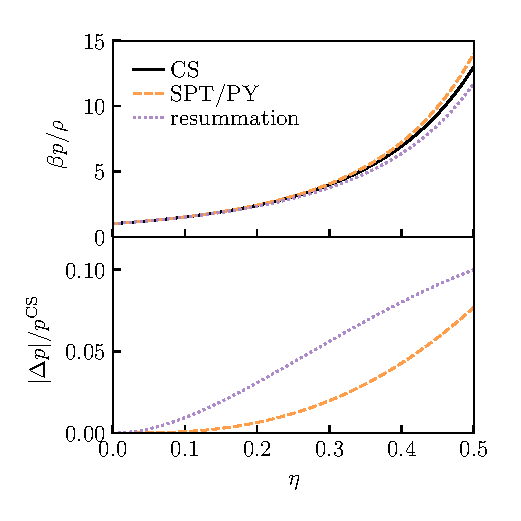
\includegraphics[width=0.9\linewidth,outer]{resummation-pressure}
  \caption[Accuracy of equation of state from partially resumming the virial series]{
    Equations of state for the single-component hard sphere liquid: Carnahan-Starling (CS), the scaled particle/Percus Yevick (SPT/PY) and the equation obtained from resumming terms in the virial series where there is a commong point of intersection.
    Top panel: pressure equations of state.
  Bottom panel: errors in the SPT/PY and resummation pressures are comparable across the whole liquid regime, taking the CS equation as the quasi-exact result.}
  \label{fig:resummation-pressure}
\end{SCfigure}

For single-component hard spheres the pressure obtained from the resummation in the previous section yields
\begin{equation}
  \frac{\beta p}{\rho} =
  \begin{cases}
    \frac{1}{1-\eta} & \; d=1 \\
    \frac{1}{(1-\eta)^2} & \; d=2 \\
    \frac{1 + \eta + (\frac{3\pi^2}{16} - 2) \eta^2}{(1-\eta)^3} & \; d=3.
  \end{cases}
\end{equation}
The resulting pressures for $d \le 2$ are identical to the scaled particle theory equations of state, where the first is the exact solution \eqref{eq:hard-rods-eos}.
For $d=3$ the resulting equation of state has a similar structure to the scaled particle theory solution (or equivalently the Percus-Yevick equation of state by the compressibility route) (SPT/PY) but it is slightly less accurate: at the freezing point $\eta_f \simeq 0.494$ the PY equation overestimates the pressure by $\sim7\%$ while for the above equation this is underestimated by $\sim11\%$, taking the Carnahan-Starling (CS) equation of state \cite{CarnahanJCP1969} as an estimate of the exact value.
The three equations of state mentioned are plotted together in Fig.\ \ref{fig:resummation-pressure} across the whole liquid regime in hard spheres.
While not exact, this shows that the morphometric contributions account for $\sim$90\% of the contributions to the equation of state which may suggest why morphological thermodynamics has been found to be highly accurate for descriptions of the hard sphere liquid \cite{RothPRL2006,LairdPRE2012,BlokhuisPRE2013,UrrutiaPRE2014,Hansen-GoosJCP2014,RobinsonPRL2019}.
This is discussed in more detail in the context of FMT in \cite{MarechalPRE2014}, and is partially attributable to cancellations of terms omitted from the resummation.

To account for the reduced accuracy of this equation of state for $d=3$ compared with PY, we observe that the PY hard sphere solution captures the third virial coefficient exactly, while this approach only provides a lower bound; the omitted configurations are known in the FMT literature as ``lost cases'' \cite{TarazonaPRE1997}.
A semi-empirical approach could reweight the final term in \eqref{eq:a3-d=3} to produce the third virial coefficient (if known), giving an equation of state for arbitrary mixtures of convex particles.
This reweighting is implicit in scaled particle theory and the Rosenfeld FMT functional \cite{TarazonaPRE1997,MarechalPRE2014}.

We see similar accuracy in the predicted surface tension at an infinite planar wall determined by $a_2$
\marginfootnote{This is true up to a normalisation constant, as $a_2$ conjugates with the intrinsic volume $V_2$ rather than the area $A = 2V_2$.
  The usual planar surface tension is thus obtained as $\gamma_\infty = a_2/2$.}.
The surface tension at an infinite planar wall is simply $a_2$ because it conjugates with the area.
In Ref.\ \cite{DavidchackMP2015} the results of extensive simulations measuring $a_2$ were parameterised by the following expression
\begin{equation}\label{eq:quasi-exact-surface-tension}
  %\begin{split}
  \beta a_2
  =
  \frac{1}{\pi \sigma^2} \left(
  \frac{\eta (2 + 3\eta - \frac{9}{5}\eta^2 - \frac{4}{5}\eta^3 - (5 \times 10^4) \eta^{20})}{(1 - \eta)^2}
  %% \right.
  %% \\
  %% &
  %% \left.
  %% \vphantom{\frac{1}{1}}
  - \ln{(1 - \eta)}
  \right),
  %\end{split}
\end{equation}
which we use to gauge the accuracy of predicted surface tensions.
We also compare the values of $a_2$ predicted by other morphometric theories of Ref.\ \cite{Hansen-GoosJPCM2006} (SPT/CS) and Ref.\ \cite{RobinsonPRE2019} (virial/CS).
The surface tensions are plotted in Fig.\ \ref{fig:resummation-a2}; the accuracy of the new result is comparable to SPT/PY in the liquid regime with the maximum error reaching $\sim12\%$.
Unsurprisingly, the other morphometric theories feature more accurate surface tensions; this is likely because they were constructed to satisfy thermodynamic relations which improves their accuracy.
%By contrast, the resummation route was not constructed for accuracy nor to satisfy thermodynamic relations.
Curiously, the error in the new theory scales almost identically to virial/CS theory at small $\eta$ even though the sign is different; all of the previous morphometric theories overestimate the surface tension, whereas the resummation route underestimates it.

\begin{SCfigure}
  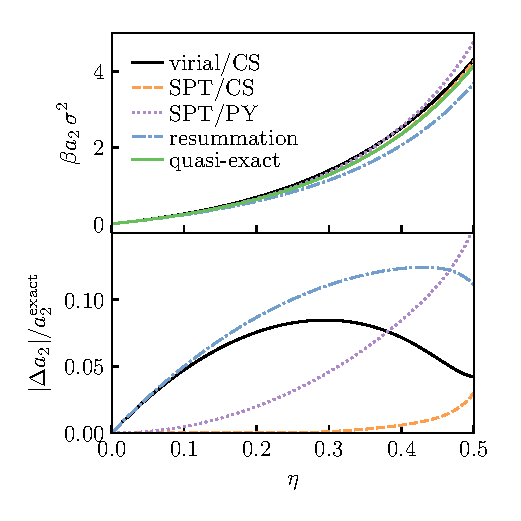
\includegraphics[width=0.9\linewidth,outer]{resummation-a2}
  \caption[Accuracy of surface tension from partially resumming the virial series]{
    Comparison of surface tensions for different morphometric theories.
  using the highly accurate result \eqref{eq:quasi-exact-surface-tension} from Ref.\ \cite{DavidchackMP2015} valid until $\eta \sim 0.5$.}
  \label{fig:resummation-a2}
\end{SCfigure}

%% \subsection{Beyond convex geometries and the choice of dividing surface}
%% \label{sec:general-geometries}

%% \begin{figure*}
%%   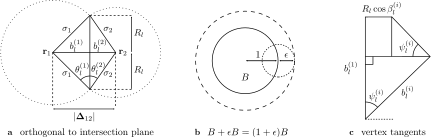
\includegraphics[width=0.65\linewidth,outer]{minkowski_addition}
%%   \caption{A dimer geometry considered in pair correlations in a fluid of $B$ particles showing (a) solute of two spheres $A$ generating an excluded volume $A \minkplus B$ and (b) the effective connected solute $A \minkplus B \minkminus B$.
%%   The exluded volume in each case is identical i.e.\ $A \minkplus B \minkminus B \minkplus B = A \minkplus B$.}
%%   \label{fig:minkowski_addition}
%% \end{figure*}

%% Until now we have focused on convex bodies, but we will now argue that the results apply for more general bodies.
%% In particular, for many-body correlations the ``solute'' consists of the disjoint union of particles see e.g.\ Fig.\ \ref{fig:system}.
%% We will determine necessary conditions for validity of the morphometric approach in in general solutes by examining the exact morphometric contributions described in previous sections.
%% A related problem is thermodynamic consistency for different choices of dividing surfaces in \eqref{eq:surface-tension}, which we will address in parallel.

%% Based on the exact results there are two ways the approach could fail:
%% \begin{enumerate}
%% \item For geometries where the integral geometric formula are invalid, e.g.\ the kinematic integrals, for non-convex geometries kinematic formula, and
%% \item Where the interaction with the solute cannot be reduced to the Euler characteristic, i.e.\ \eqref{eq:interactions-euler-equivalence}.
%% \end{enumerate}
%% As there are exact morphometric contributions to the free energy, a good approximation scheme should contain these; conversely, where these contributions are not captured provides necessary conditions for the scheme's validity.
%% We will address both potential failures in turn.

%% We used the kinematic integral \eqref{eq:binomial-kinematic-equation}, and its iterated form \eqref{eq:multinomial-kinematic-equation}, with convex bodies but it is valid for many more physically relevant geometries.
%% They can be extended \cite{Klain1997} to so-called \emph{polyconvex} bodies (also known as the convex ring), meaning any body formed by the countable union of convex objects.
%% This latter category covers most physically meaningful geometries, omitting pathological cases where size measures lose their meaning creating paradoxes \cite{BanachFM1924}.
%% The argument from Hadwiger's theorem similarly extends to polyconvex bodies.

%% Though the integral theorems hold for geometries of relevant physical interest, the equivalence between interaction and geometry \eqref{eq:interactions-euler-equivalence} may not.
%% We will consider two examples below in order to extend the geometric formalism to cases of physical interest.

%% First, consider the geometry formed by creating an infinitesimally small cavity inside a convex object.
%% Its Euler characteristic will deviate by $\pm 1$ (with sign dependent on dimension), however the interactions are unchanged because the cavity is not large enough to contain a finite-sized object.
%% In this case \eqref{eq:interactions-euler-equivalence} holds so long as the original convex geometry is used in place of the `true' body with the cavity.
%% %Going a step further, for finite-sized cavities able to contain a solvent particle, the cavity will be dynamically inaccessible to solvent particles (unless initially prepared inside) so the whole body can be treated as if it were solid, i.e.\ the interior of $\partial B$.

%% Next, we consider a geometry more typical of correlations in liquids: a dimer formed by two unit balls a distance $r$ apart i.e.\
%% \begin{equation*}
%%   A(r) = B^d \cup \mathcal{T}(r) B^d,
%% \end{equation*}
%% sketched in Fig.\ \ref{fig:minkowski_addition}.
%% This geometry is non-convex, and for $r > 1$ it is not even simply connected.
%% For interactions with a convex solvent particle $B$ we have possible Euler characteristics of intersection $\chi(A \cap B) \in \{0, 1, 2\}$ whereas $e^{-\beta u(A, B)} \in \{0, 1\}$, so it is not possible to establish an exact correspondence between the two.
%% We can proceed by determining an effective geometry where this relation does hold.
%% The exact result \eqref{eq:exact-mayer-exclusion} can be written
%% \begin{equation}
%%   \begin{split}
%%     e^{-\beta u(A, \mathcal{T} B)} - 1
%%     &= -\chi((A \minkplus B) \cap \{\vec{r}\}) \\
%%     &= -\chi((A \minkplus B \minkminus B) \cap B),
%%   \end{split}
%% \end{equation}
%% with the last line valid so long as $A \minkplus B \minkminus B = \{\vec{c} \, | \, (\vec{c} \minkplus B) \subseteq A \minkplus B\}$ is simply connected, otherwise the Euler characteristic of the intersecting geometry can be greater than one $\chi((A \minkplus B \minkminus B) \cap B) > 1$.
%% The effective geometry $A \minkplus B \minkminus B$ recovers the correspondence between interaction and geometry \eqref{eq:interactions-euler-equivalence}.
%% Addition (dilation) and subtraction (erosion) operations are not inverse operations so $A \minkplus B \minkminus B \ne A$, however $A \minkplus B \minkminus B \minkplus B = A \minkplus B$ so $A \minkplus B \minkminus B$ acts as an effective generator of the exclusion region.
%% The effective geometry for the previous example, a nearly convex body with an infinitesimal cavity, recovers the convex object.

%% Related to the above discussion is the effect of the choice of dividing surface on the decomposition of surface and volume terms in \eqref{eq:surface-tension}.
%% The thermodynamics should not depend on the choice of boundary, i.e.\ we can define a functional working with the parallel surface
%% \begin{equation*}
%%   \Delta \Omega'[A \minkplus \epsilon B]
%%   =
%%   \sum_{k=0}^d a_k' V_k(A \minkplus \epsilon B)
%% \end{equation*}
%% but thermodynamic consistency requires
%% \begin{equation*}
%%   \Delta \Omega[A] =
%%   \Delta \Omega'[A \minkplus \epsilon B].
%% \end{equation*}
%% A controlled expansion of the solvation energy which allows for different choices of dividing surface must be invariant to the particular choice.
%% The transformation between the coefficients $\{a_k\}$ and $\{a'_k\}$, which we give explicitly in Appendix~\ref{appendix:parallel-surfaces}, are straightforward which is a particular strength of using the morphometric \emph{ansatz}.
%% When this transformation fails leading to inconsistent thermodynamics, we know the theory has failed.
%% We find a necessary condition for the theory's validity is thus that $\chi(A \minkplus B^d \minkminus B^d) = \chi(A \minkplus B^d)$.

%% The boundary of the effective volume $\partial(A \minkplus B \minkminus B)$ is commonly called the \emph{molecular surface} \cite{?}, while the boundary of the excluded volume $\partial(A \minkminus B)$ is referred to as the \emph{solvent accessible surface}.
%% There is also an infinite family of equivalent parallel surfaces in between i.e.\ $\partial(A \minkplus B \minkminus \epsilon B)$ for $\epsilon \in [0, 1]$ but the two extremes are the most natural choices.
%% When the boundary of the effective geometry (molecular surface) self-intersects, we expect the theory to break down.
%% In the previous example this occurs at $r = 2\sqrt{3}$ for spherical solvent particles $B = B^d$ \cite{OettelEL2009}.
%% At this point, descriptions with different choices of boundary become inconsistent.
%% Consider the Euler characteristic of the effective body (molecular surface)
%% \begin{equation}
%%   \chi(A \minkplus B^d \minkminus B^d)
%%   =
%%   \begin{cases}
%%     1 & r < 2\sqrt{3} \\
%%     2 & r > 2\sqrt{3}
%%   \end{cases}
%% \end{equation}
%% whilst for the parallel volume (solvent accessible surface)
%% \begin{equation}
%%   \chi(A \minkplus B^d)
%%   =
%%   \begin{cases}
%%     1 & r < 2 \\
%%     2 & r > 2
%%   \end{cases}
%% \end{equation}

\section{Discussion}

%We have derived the morphometric solvation free energy for mixtures of hard convex particles from first-principles using the virial series.

While the morphometric theory we have derived from the virial series is less accurate than theories obtained from other routes. 
Specifically, in $d=3$ the pressure and surface tension is comparable in accuracy to the classic SPT/PY route and in $d=2$ the two approaches are equivalent.
\todo{Check that surface tension in $d=2$ is the same as SPT.}
However, the usefulness of the new route is extends beyond mere accuracy; the free energy we have identified emerges \emph{rigorously} as a contribution from the virial series.
The fact that this exact contribution is still reasonably accurate suggests that the corrections to it are small, providing further justification of the morphometric approach.
This means we could write the insertion cost for a solute $K$ as the \emph{exact} decomposition
\begin{equation}\label{eq:exact-morph-decomposition}
  \Delta \Omega[K]
  =
  \sum_{k=0}^d a_k V_k(K)
  + \Delta \Omega_\mathrm{extra}[K]
\end{equation}
with coefficients $a_k$ as previously calculated, and $\Delta \Omega_\mathrm{extra}$ contains the remaining contributions.
Notably the exponentially damped oscillations occuring in pair correlations at asymptotically large separations must be contained within $\Delta \Omega_\mathrm{extra}$.
The insertion cost is known to contain singularities \cite{ReissJCP1959} so it is unlikely that $\Delta \Omega_\mathrm{extra}$ possesses a simple analytic form.
It is possible that additional exact morphometric contributions exist, and they would be contained in $\Delta \Omega_\mathrm{extra}$ also.

Furthermore, the formal derivation we have followed naturally leads to explicit expressions for $\Delta \Omega_\mathrm{extra}$.
The next leading contribution from the virial series would be:
\begin{equation}
  \Delta \Omega_\mathrm{extra}[K]
  =
  \frac{\rho^2}{2}
  \sum_{s_1=1}^m \sum_{s_2=1}^m
  x_{s_1} x_{s_2}
  \left(
  \int_{G_d^2} \chi(K \cap g_1 K_{s_1}) \chi(K \cap g_2 K_{s_2}) \chi(g_1 K_{s_1} \cap g_2 K_{s_2}) dg_1 dg_2
  - \Lambda_{s_1,s_2} \right)
  + \mathcal{O}(\rho^3),
\end{equation}
which involves a \emph{ring integral}.
These integrals can be calculated straightforwardly in hard spheres \cite{MontrollJCP1941}, or using the Radon transform for convex geometries of arbitrary shapes \cite{WertheimMP1994,WertheimMP1996,WertheimMP1996a}.
Corrections could be systematically included by further resummations over topologically identical integrations, with ring integrals as the leading order terms.
The integral corrections are discussed in Ref.\ \cite{MarechalPRE2014} in the context of free energy functionals for inhomogeneous liquids; our system is effectively homogeneous so we expect it to be easier to construct a theory with higher-order terms.

The form of the exact contribution is instructive in how it applies to mixtures.
It is argued in Ref.\ \cite{KodamaJCP2011} that for an $m$-component mixture the appropriate morphometric form reads
\begin{equation}\label{eq:morphometric-approach-mixtures}
  \Delta \Omega
  =
  \sum_{i=1}^m
  a_3^{(i)} V_i
  + a_2^{(i)} A_i
  + a_1^{(i)} C_i
  + a_0^{(i)} X_i
\end{equation}
where the coefficients $a_k^{(i)}$ now depend on the specific interactions with each species and their composition, and $\{V_i, A_i, C_i, X_i\}$ are geometric measures on some composite body of the solute with solvent particles of species $i$, e.g.\ their specific exluded volume.
By contrast, our exact morphometric contribution does not involve different intrinsic volumes for the different cross-species interactions, suggesting \eqref{eq:morphometric-approach} is a general enough \emph{ansatz} and the extension for mixtures \eqref{eq:morphometric-approach-mixtures} proposed in Ref.\ \cite{KodamaJCP2011} may be unnecessary.

In addition to the accuracy of the exact contribution, we can argue against the alternative morphometric form for mixtures \eqref{eq:morphometric-approach-mixtures} by considering the polydisperse mixture limit.
The alternative form contains $4m$ parameters which becomes underconstrained in the polydisperse limit $m \to \infty$, so it is unlikely that the coefficients $a_k^{(i)}$ can be totally independent.
More precisely, thermodynamic consistency of the (osmotic) pressure requires
\begin{equation}\label{eq:osmotic-consistency-1}
  \begin{split}
    \beta p
    &=
    \rho - \beta f^\mathrm{ex}
    + \rho \left( \frac{\partial \beta f^\mathrm{ex}}{\partial \rho} \right)_{V,T}
    \\
    &=
    \rho - \beta f^\mathrm{ex}
    + \rho \sum_{i=1}^m
    x_i \left( \frac{\partial \beta f^\mathrm{ex}}{\partial x_i} \right)_{V,T}
  \end{split}
\end{equation}
where $f^\mathrm{ex} = F^\mathrm{ex}/V$ is the (excess) free energy density.
The latter line, valid in the case of mixtures, becomes poorly defined in the polydisperse limit $m \to \infty$ with $x_i \to 0$.
To remain well-defined for polydisperse systems the composition dependence of the free energy should reduce to a (finite) set of \emph{weighted densities} \cite{GualtieriJCP1982, WarrenPRL1998, SollichPRL1998, SollichAiCP2001}.
This is the case for our virial-derived approach where the density dependence enters through scaled particle variables $\{\xi_k\}$, so \eqref{eq:osmotic-consistency-1} becomes
\begin{equation}\label{eq:osmotic-consistency-2}
  \beta p
  =
  \rho - \beta f^\mathrm{ex}
  + \sum_k
  \xi_k \left( \frac{\partial \beta f^\mathrm{ex}}{\partial \xi_k} \right)_{V,T}.
\end{equation}
To demonstrate that our form works for both discrete and continuous (polydisperse) mixtures, we rewrite the geometric parameters \eqref{eq:spt-variables} in the more general form
\begin{equation}
  \xi_k
  =
  \rho \int \widetilde{V}_k(K_s) d\mu(s),
\end{equation}
introducing the probability measure $\mu(s)$ for the molarities of particle species/shapes such that $\int d\mu(s) = 1$.
This reduces to the previous form for discrete mixtures if we set $\mu(s)$ to the counting measure, however in integral form we are free to extend the calculation to continuous mixtures.

As an example we consider a polydisperse mixture of particles of reference shape $K$ with uniformly distributed sizes $s \in [s_0, s_1]$ giving $V_k(K_s) = V_k(s K) = s^k V_k(K)$, then
\begin{equation}
  \begin{split}
    \xi_k
    &=
    \rho \widetilde{V}_k(K) \int_{s_0}^{s_1} s^k ds
    \\ &=
    \rho \widetilde{V}_k(K) \left(\frac{s_1^{k+1} - s_0^{k+1}}{k+1}\right).
  \end{split}
\end{equation}
Inserting this reweighted volume into the explicit expressions given in the appendix yields new thermodynamic coefficients for uniformly distributed polydisperse mixtures.
The composition dependence enters only through moments of the size distribution guaranteeing a well-defined free energy, detailed discussion of which can be found in Refs.\ \cite{GualtieriJCP1982,WarrenPRL1998,SollichPRL1998,SollichAiCP2001}.

\section{Summary}

We have derived an exact morphometric contribution for a general class of hard particle liquids by resumming terms in the virial series.
Previous studies have primarily used FMT to develop morphometric theories, so we have successfully developed an independent justification for the morphometric approach as the leading term in a controlled expansion.
The exact result applies for mixtures of hard convex particles in an isotropic phase.

%This result is not that surprising as the morphometric approach can be obtained as a limit case of FMT \cite{Hansen-GoosJPCM2006}, which itself can be formulated as the resummation of the same terms in the virial expansion \cite{LeithallPRE2011,KordenPRE2012,MarechalPRE2014}.

In hard spheres the exact contribution features similar accuracy as scaled particle theory, so it captures most contributions to the bulk free energy and seems to be why the approach has been successful.
Though as noted in Ref.\ \cite{MarechalPRE2014} this is partially due to a cancellation in the omitted terms of the virial expansion, so it may still desirable to improve the morphometric approach by inclusion of additional terms.
The exact morphometric contribution provides a suitable starting point for including additional terms to improve accuracy.

%\appendix*

\section{Explicit morphometric contributions in the virial expansion}
%\label{appendix:lambda}

Here we explicitly evaluate the contributions in the virial expansion from configurations sharing a common point of intersection via \eqref{eq:little-lambda}.

For $d=1$ the index runs over $k \in \{0,1\}$, giving condition on the summation indices $N_0 = k$ and $N_1 = n - N_0$ leading to a single term for each value of $k$:
\begin{subequations}
  \label{eq:little-lambda-d=1}
  \begin{align}
    \lambda_0^{(n)} &= \xi_1^n
    \\
    \lambda_1^{(n)} &= n \xi_0 \xi_1^{n-1}.
  \end{align}
\end{subequations}
For $d=2$ we have $k \in \{0,1,2\}$, with summation conditions $2N_0 + N_1 = k$ and $N_2 = n - N_1 - N_0$ giving:
\begin{subequations}
  \label{eq:little-lambda-d=2}
  \begin{align}
    \lambda_0^{(n)} &= \xi_2^n
    \\
    \lambda_1^{(n)} &= n \xi_1 \xi_2^{n-1}
    \\
    \lambda_2^{(n)} &=
    n \xi_0 \xi_2^{n-1}
    + \frac{n(n-1)}{2} \xi_1^2 \xi_2^{n-2}.
  \end{align}
\end{subequations}
Finally, for $d=3$ we have $k \in \{0,1,2,3\}$, with summation conditions $3N_0 + 2N_1 + N_2 = k$ and $N_3 = n - N_2 - N_1 - N_0$ giving:
\begin{subequations}
  \label{eq:little-lambda-d=3}
  \begin{align}
    \lambda_0^{(n)} &= \xi_3^n
    \\
    \lambda_1^{(n)} &= n \xi_2 \xi_3^{n-1}
    \\
    \lambda_2^{(n)} &=
    n \xi_1 \xi_3^{n-1}
    + \frac{n(n-1)}{2} \xi_2^2 \xi_3^{n-2}
    \\
    \lambda_3^{(n)} &=
    n \xi_0 \xi_3^{n-1}
    + n(n-1) \xi_1 \xi_2 \xi_3^{n-2}
    \nonumber \\ & \qquad
    + \frac{n(n-1)(n-2)}{6} \xi_2^3 \xi_3^{n-3}.
  \end{align}
\end{subequations}

We will now resum $\lambda_k^{(n)}$ over $n$ in order to determine the values of $a_k$ for $d \le 3$.
For $d=1$ we insert \eqref{eq:little-lambda-d=1} into \eqref{eq:final-a-coefficient}:
\begin{subequations}
  \begin{align}
    \beta a_0
    &= - \ln{(1 - \eta)},
    \\
    \beta p =
    \beta a_1 &=
    \frac{2 \xi_0}{1-\eta},
  \end{align}
\end{subequations}
with $\xi_0 = \rho / 2$ giving the exact result for hard rods \eqref{eq:hard-rods-morphometric} and \eqref{eq:hard-rods-eos}.
For $d=2$ we insert \eqref{eq:little-lambda-d=2} into \eqref{eq:final-a-coefficient}:
\begin{subequations}
  \begin{align}
    \beta a_0 &= -\ln{(1 - \eta)},
    \\
    \beta a_1 &= \frac{2 \xi_1}{1-\eta},
    \\
    \beta p =
    \beta a_2 &=
    2\pi \left(
    \frac{\xi_0}{1-\eta}
    + \frac{\xi_1^2}{2(1-\eta)^2}
    \right).
  \end{align}
\end{subequations}
Note: for hard discs of diameter $\sigma$ we obtain $V_1 = \pi \sigma / 2$ so $\xi_0 = \rho / (2\pi)$ and $\xi_1 = \rho \sigma / 2$ for the single-component fluid.
Finally, for $d=3$ we insert \eqref{eq:little-lambda-d=3} into \eqref{eq:final-a-coefficient}:
\begin{subequations}
  \begin{align}
    \beta a_0 &= -\ln{(1 - \eta)},
    \\
    \beta a_1 &= \frac{2 \xi_2}{1-\eta},
    \\
    \beta a_2 &=
    2 \pi
    \left(
    \frac{\xi_1}{1-\eta}
    + \frac{\xi_2^2}{2(1-\eta)^2}
    \right),
    \\
    \beta p =
    \beta a_3 &=
    8 \pi\left(
    \frac{\xi_0}{1-\eta}
    + \frac{\xi_1 \xi_2}{(1-\eta)^2}
    + \frac{\xi_2^3}{3 (1-\eta)^3}
    \right).
    \label{eq:a3-d=3}
  \end{align}
\end{subequations}
Note: for hard spheres of diameter $\sigma$ we obtain $V_1 = 2\sigma$ and $V_2 = \pi \sigma^2 / 2$ so $\xi_0 = \rho / (8\pi)$, $\xi_1 = \rho \sigma / (2\pi)$ and $\xi_2 = \rho \pi \sigma^2 / 8$ for the single-component fluid.
In the above steps we have used the fact that $\xi_d = \eta$ to simplify the resulting expressions.

\ifdefined\includebibliography
  \printbibliography
\fi

\end{document}
